\documentclass[final]{beamer}
\mode<presentation>

% STEP 1: Change the next line according to your language
\usepackage[brazil]{babel}

% STEP 2: Make sure this character encoding matches the one you save this file as
% (this template is utf8 by default but your editor may change it, causing problems)
\usepackage[utf8]{inputenc}

% You probably don't need to touch the following four lines
\usepackage[T1]{fontenc}
\usepackage{lmodern}
\usepackage{amsmath,amsthm, amssymb, latexsym}
\usepackage{exscale} % required to scale math fonts properly

\usepackage[orientation=portrait,size=a0,scale=1.4]{beamerposter}

\usepackage{subcaption}
\usepackage{graphicx}


% STEP 3:
% Change colours by setting \usetheme[<id>, twocolumn]{HYposter}.
\usetheme[cic, twocolumn]{HYposter}
% The different ids are:
%  cic: Departamento de ciencia da computacao unb
%  maa: Faculty of Agriculture and Forestry 
%  hum: Faculty of Arts 
%  kay: Faculty of Behavioural Sciences 
%  bio: Faculty of Biological and Environmental Sciences 
%  oik: Faculty of Law 
%  med: Faculty of Medicine 
%  far: Faculty of Pharmacy 
%  mat: Faculty of Science 
%  val: Faculty of Social Sciences 
%  teo: Faculty of Theology 
%  ell: Faculty of Veterinary Medicine 
%  soc: Swedish School of Social Science 
%  kir: University of Helsinki Library
%  avo: Open University
%  ale: Aleksanteri Institute
%  neu: Neuroscience Institute
%  biot: Bioscience Institute
%  atk: Computer centre
%  rur: Ruralia Institute
%  koe: Laboratory animal centre
%  kol: Collegium for Advanced Studies
%  til: Center for Properties and Facilities
%  pal: Palmenia
%  kie: Language centre
% Without options a black theme without faculty name will be used.


% STEP 4: Set up the title and author info
\titlestart{Avaliação Institucional} % first line of title
\titleend{IFB - Campus São Sebastião} % second line of title
% \titlesize{\Huge} % Use this to change title size if necessary. See README for details.

%\author{First Author$^1$, \\ Second Author$^2$}
%\institute{$^1$Some Institute, \url{email.address@institute}, \\ $^2$Another Institute}

\author{A. Beatriz ~ F.L. Pinheiro ~ M. Gabriel ~ T. Brunacci ~ V. Henrique}
%\institute{Departamento de Planejamento e Administração - PAD \url{http://www.fe.unb.br/}}


% Stuff such as logos of contributing institutes can be put in the lower left corner using this
%\leftcorner{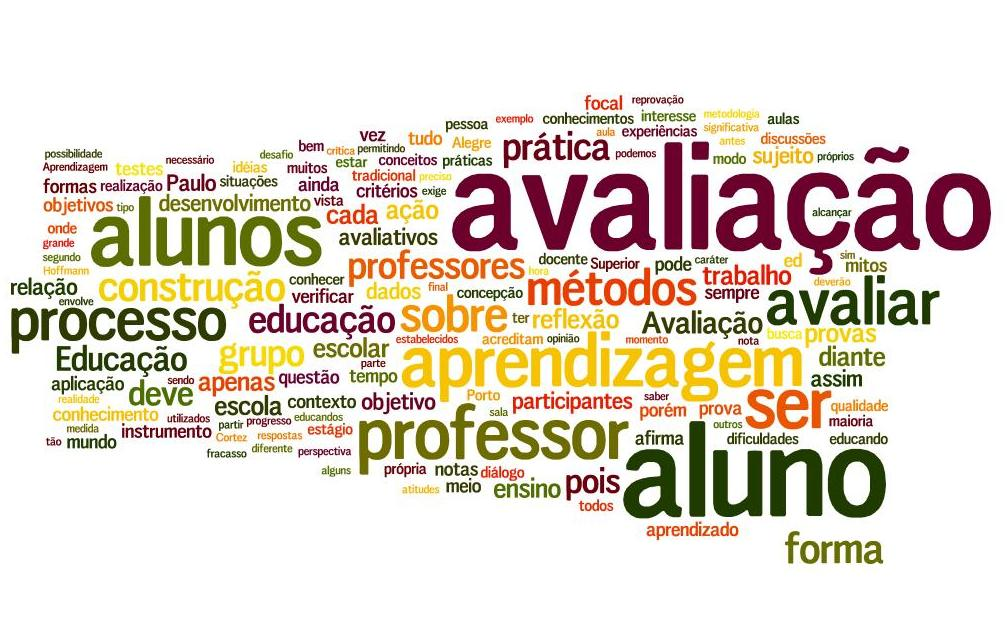
\includegraphics[width=\columnwidth]{cloud.jpg}}


\begin{document}

\begin{poster} 
% First column
\newcolumn

\section{O que é?}

A avaliação institucional é um processo de pesquisa e de comunicação que visa proporcionar uma reflexão contínua e revisar permanentemente a\\ atuação da Instituição, tendo em vista o alcance de sua missão, de seus objetivos e o aprimoramento da qualidade institucional.  Ela avalia o\\ contexto escolar numa visão abrangente do processo educativo, de modo a permitir a identificação das fragilidades e potencialidades da unidade escolar,\\ a fim de promover uma reflexão e discussão, com vistas à melhoria da qualidade social da educação.

\section{Por que avaliar?}
Esse processo objetiva identificar fatores que interferem positiva ou negativamente no desempenho da Instituição, fornecendo subsídios para a compreensão da realidade institucional, favorecendo as gestões acadêmica e administrativa.

\begin{figure}%
\centerline{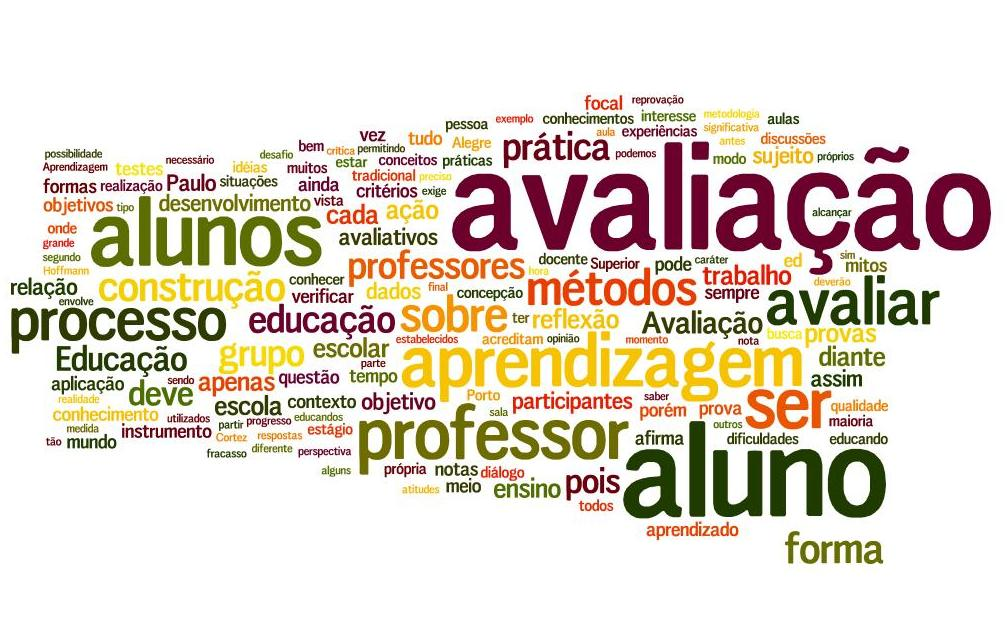
\includegraphics[width=.3\columnwidth]{cloud}}
\caption{A partir de 2004, a Avaliação Institucional passou a ser uma exigência do Governo Federal, por meio da Lei nº 10.861, de 14/04/04, que implantou o Sistema Nacional de Avaliação da Educação Superior – SINAES.}%
%\label{}%
\end{figure}

\section{O que é SINAES?}
\begin{itemize}
	\item O SINAES é parte de uma política de governo voltada à Avaliação da Educação Superior.
	\item É um sistema de avaliação global e integrado das atividades institucionais, composto por:
	\item Avaliação das Instituições de Educação Superior (AVALIES); 
	\item Avaliação dos Cursos de Graduação (ACG); 
	\item Avaliação do Desempenho dos Estudantes (ENADE). 
	\item É obrigatório em todas as instituições de ensino superior do País.
\end{itemize}

\section{Quais são os processos?}
A autoavaliação compõem-se dos seguintes processos:
\begin{itemize}
	\item Planejamento;
	\item Avaliação, Estudos e Levantamentos;
	\item Comunicação e Envolvimento da Comunidade Institucional / Acadêmica;
	\item Coordenação e Articulação da Avaliação Institucional / CPA / SINAES.
\end{itemize}

\begin{figure}%
\begin{subfigure}{\textwidth}
\centering
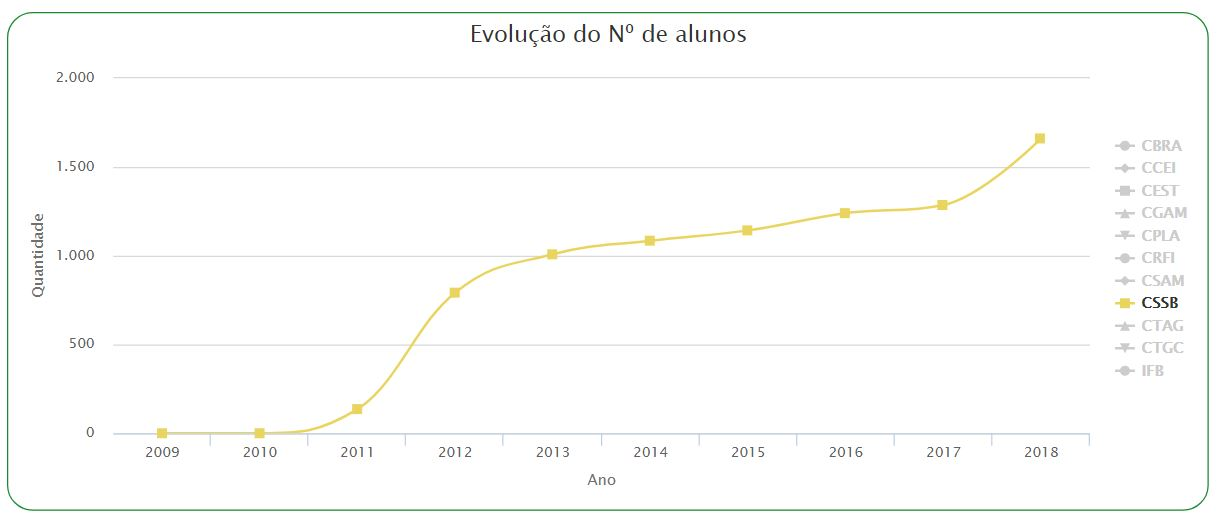
\includegraphics[width=.45\columnwidth]{alunos}
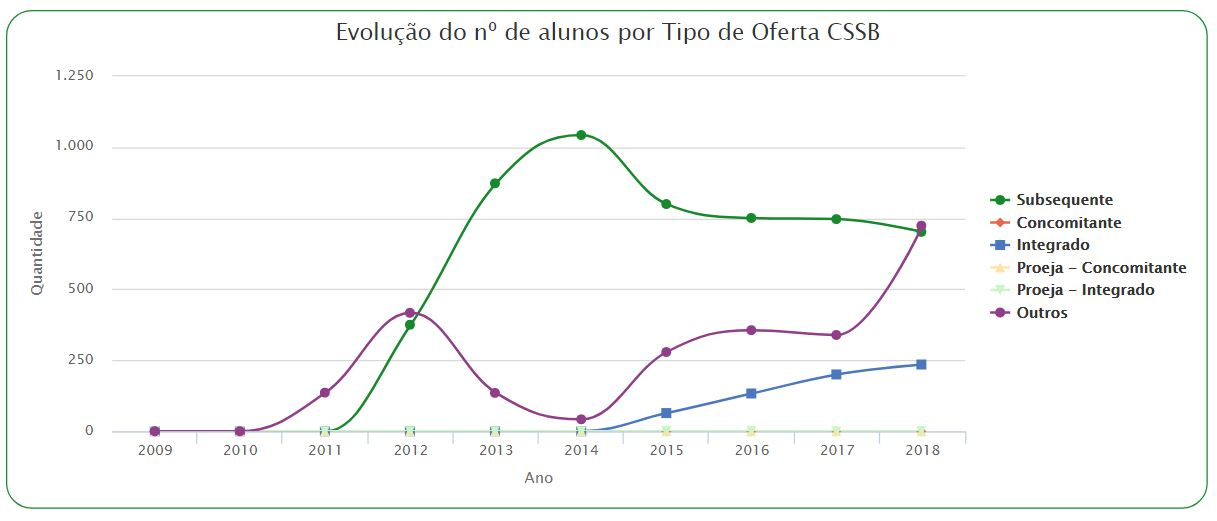
\includegraphics[width=.45\columnwidth]{oferta}
\end{subfigure}
\begin{subfigure}{\textwidth}
\centering
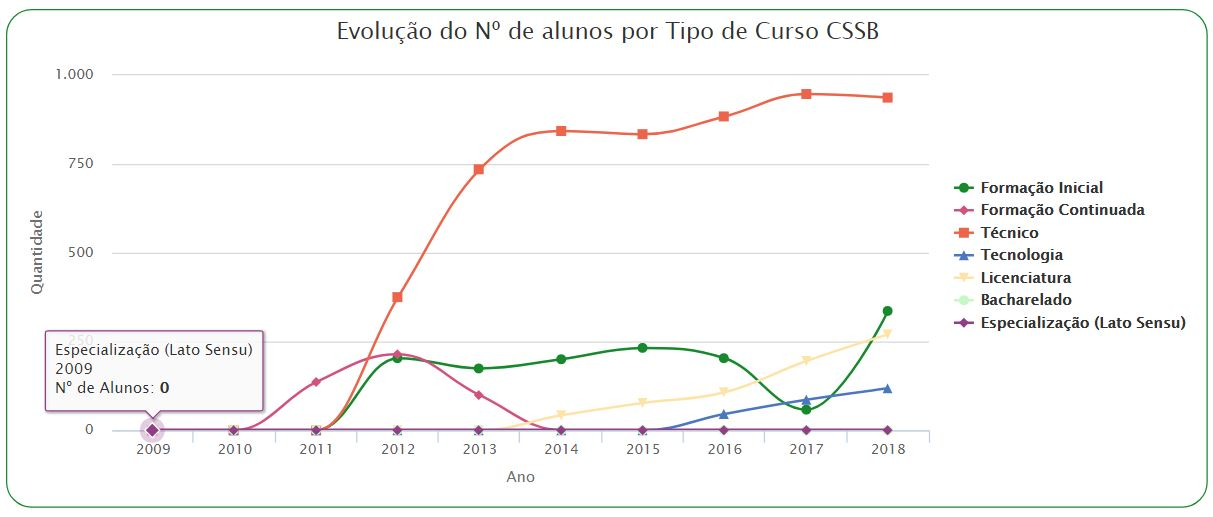
\includegraphics[width=.45\columnwidth]{tipo}
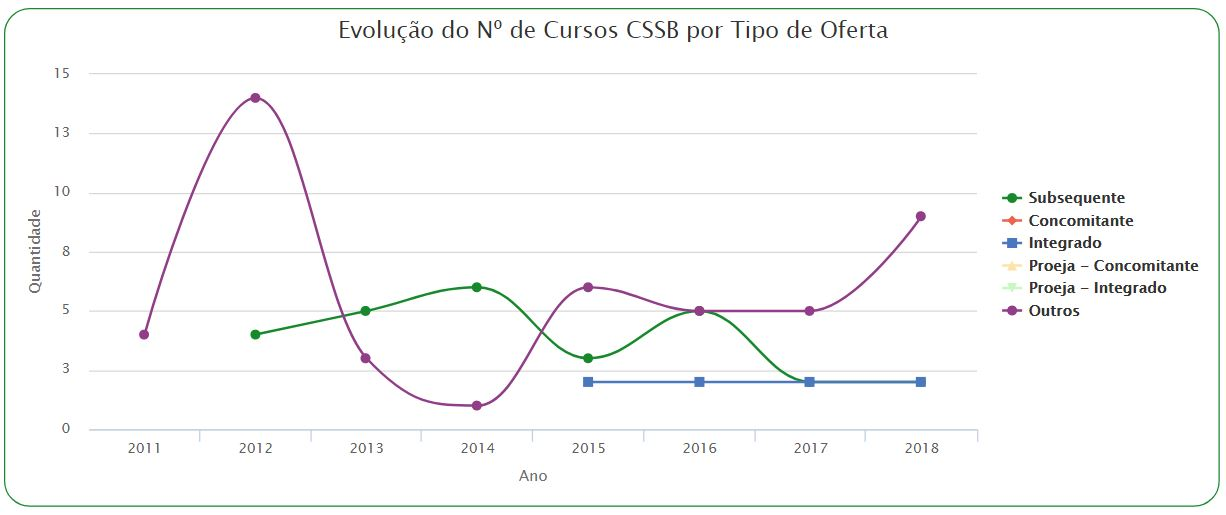
\includegraphics[width=.45\columnwidth]{cursos}
\end{subfigure}
\caption{Exemplo de dados coletados durante uma avaliação Institucional}
\end{figure}

% Second column
\newcolumn

%O que fundamenta e orienta tais processos? Como se realizam?
\section{Fundamentação}
A fundamentação teórico-metodológica do processo autoavaliativo ancoram-se nos paradigmas: crítico-dialético, sócio-antropológico e empírico-analítico, os quais definem seus procedimentos metodológicos.

Os paradigmas citados indicam ações nas abordagens:

\textbf{Quantitativa:} que consiste na aplicação de instrumentos avaliativos centralizados nos conceitos / medidas (notas), nos quais se destacam os projetos:
Avaliação no Ensino de Graduação Institucional / Cursos; 
Avaliação no Ensino de Graduação na Modalidade a Distância – EaD Institucional / Cursos. 

\textbf{Qualitativa:} que consiste em obter opiniões, informações, sugestões, avaliações por meio de ações específicas centralizadas no diálogo ou em colocações livres, em que se destacam:
Comunicações diretas, gráficas ou on-line da Avaliação Institucional e CPA; 
Reuniões de conselhos, colegiados de cursos, encontros, reuniões, outros. 
Tais abordagens interagem na análise e elaboração dos resultados finais dos projetos e ações realizados no processo autoavaliativo.


%Como é a estrategia da avaliação institucional nas escolas publicas no DF ?
\section{Estrategias no DF}
A estratégia da avaliação institucional é a integração das informações da base de dados da SEEDF (iEducar e outros) e demais dados obtidos por meio da coleta eletrônica de instrumentos de pesquisa, de modo a permitir o tratamento, cruzamento, análise das variáveis de interesse e suas correlações disponibilizando, assim, os resultados no menor espaço de tempo possível.

Após a coleta de dados será realizada uma análise descritiva, uma fotografia de como a escola se encontra. Posteriormente, serão utilizados os pressupostos da análise inferencial onde se observará a associação entre as variáveis coletadas permitindo, desta forma, conhecer a partir dos dados obtidos o perfil das unidades escolares da rede pública do Distrito Federal.




\section{Utilização dos Resultados}
%Utilização esperada dos resultados
Os resultados da Avaliação Institucional subsidiarão a reflexão de toda a comunidade escolar quanto à atuação da unidade escolar e seu projeto político-pedagógico, bem como as suas relações com a comunidade, sinalizando possíveis disfunções no seu cotidiano, de modo a viabilizar o aperfeiçoamento do exercício da Gestão Democrática e a adequação das políticas públicas educacionais.

Com a finalidade de potencializar a autoavaliação e articular seus resultados com os demais níveis de avaliação, a Coordenação de Avaliação Educacional/Gerência de Avaliação Institucional fornecerá subsídios às unidades escolares, de modo a promover reflexões norteadoras de ações que contribuam com o processo de aprendizagem.

Os resultados da avaliação institucional serão divulgados por meio de relatórios eletrônicos, por unidade escolar e Coordenação Regional de Ensino.





\begin{figure}%
\begin{subfigure}{\textwidth}
\centering
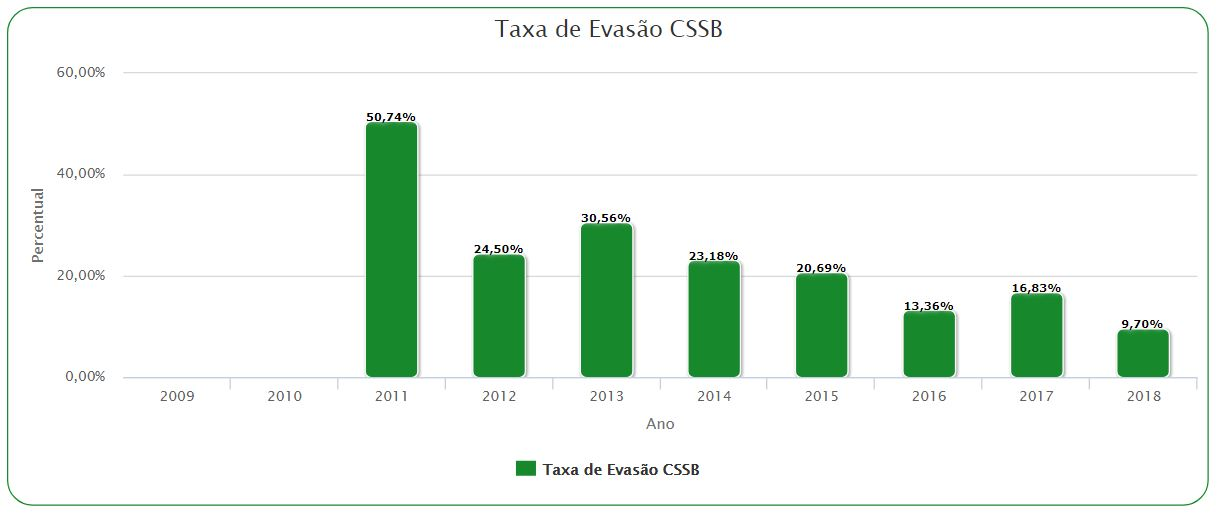
\includegraphics[width=.45\columnwidth]{evasao}
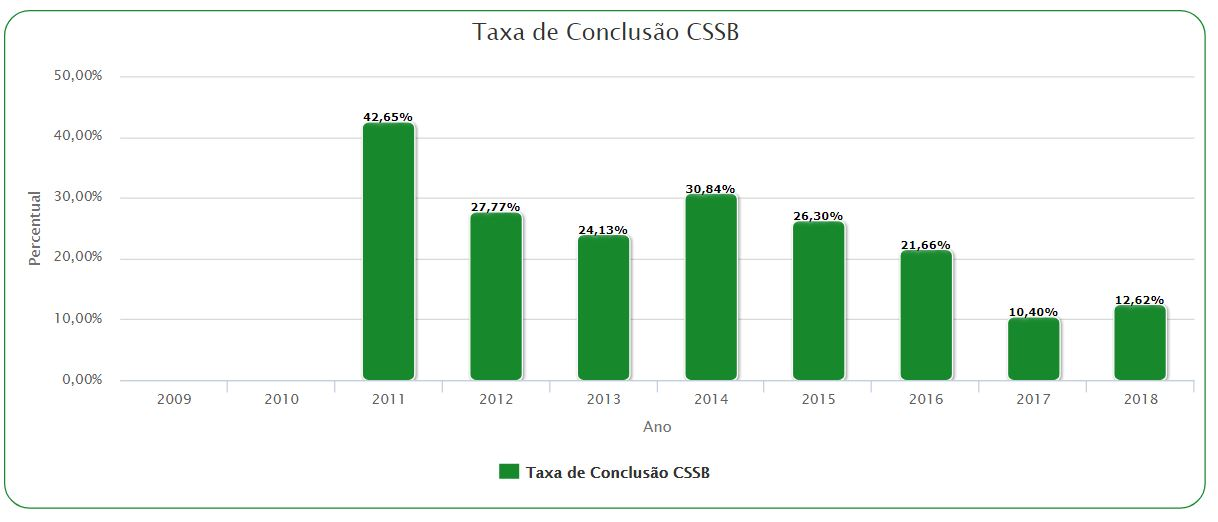
\includegraphics[width=.45\columnwidth]{conclusao}
\end{subfigure}
\begin{subfigure}{\textwidth}
\centering
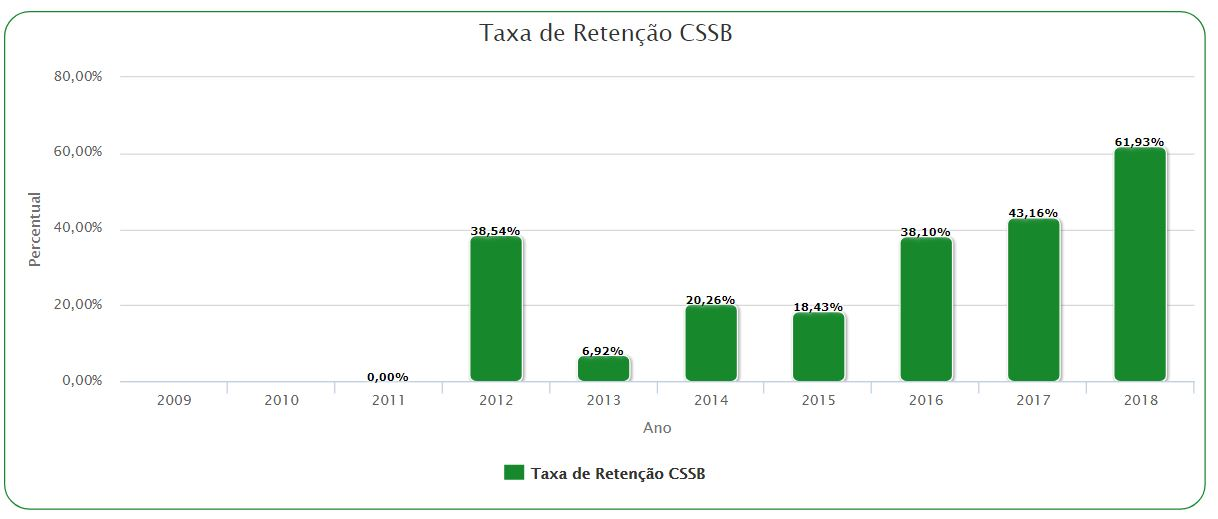
\includegraphics[width=.45\columnwidth]{retencao}
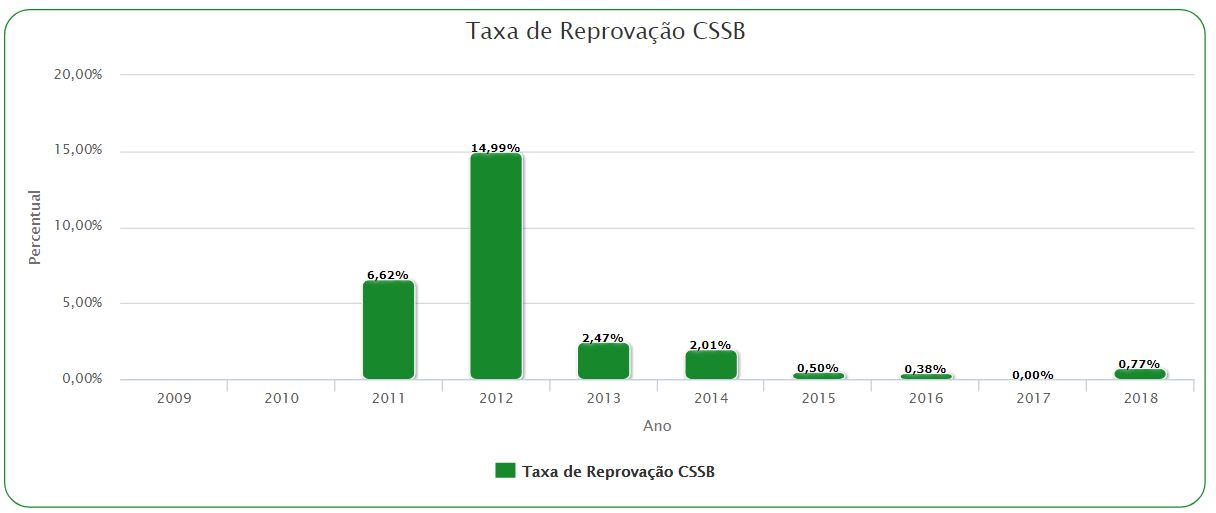
\includegraphics[width=.45\columnwidth]{reprovacao}
\end{subfigure}
\caption{Exemplo de dados coletados durante uma avaliação Institucional}
\end{figure}

%
%\bibliographystyle{abbrv}
  %\bibliography{reference}	

\end{poster}

\end{document}